\begin{figure}[ht]
\centering
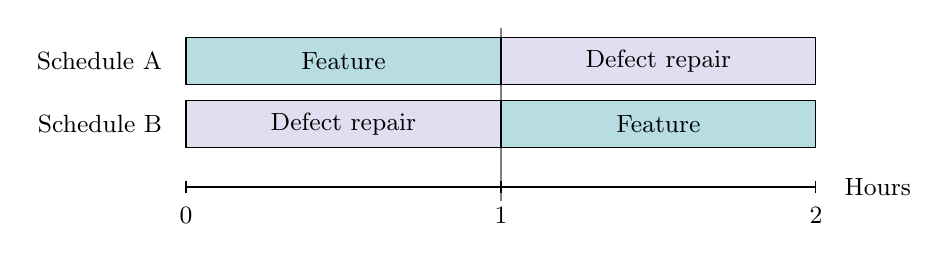
\begin{tikzpicture}[x=4.0cm,y=.8cm,font=\small]
  \definecolor{feature}{HTML}{B7DDE3}
  \definecolor{repair}{HTML}{E1DEF1}
  \draw[gray] (1,.15) -- (1,2.9);
  \draw[fill=feature] (0,2) rectangle (1,2.75);
  \draw[fill=repair] (1,2) rectangle (2,2.75);
  \draw[fill=repair] (0,1) rectangle (1,1.75);
  \draw[fill=feature] (1,1) rectangle (2,1.75);
  \node[anchor=east] at (-.045,2.375) {Schedule A};
  \node[anchor=east] at (-.045,1.375) {Schedule B};
  \node at (.5,2.375) {Feature};
  \node at (1.5,2.375) {Defect repair};
  \node at (.5,1.375) {Defect repair};
  \node at (1.5,1.375) {Feature};
  \draw (0,.38) -- (2,.38);
  \foreach \x in {0,1,2} {
    \draw (\x,.28) -- (\x,.48);
    \node[below=1.5pt] at (\x,.28) {\x};
  }
  \node[anchor=west] at (2.06,.38) {Hours};
\end{tikzpicture}
\caption{Two schedules consistent with one hour of feature work and one hour of repair by the same engineer. The first hour contains one person-hour in either schedule.}
\label{fig:shared-time}
\end{figure}
